
\vspace{-10 mm}
\begin{IEEEbiography}[{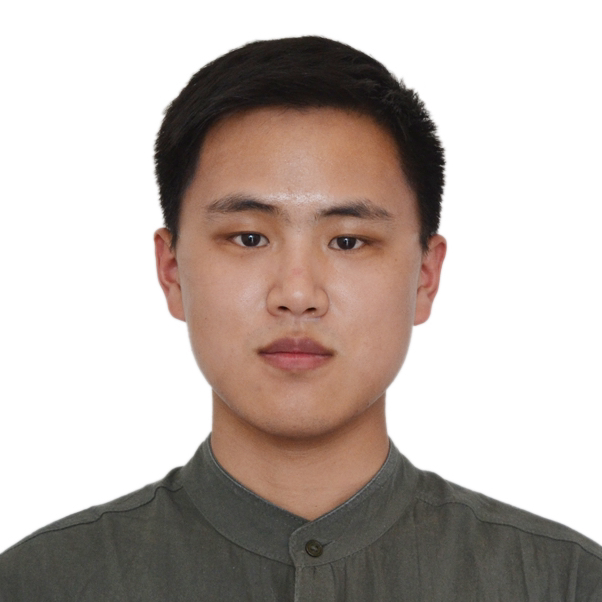
\includegraphics[width=1in,height=1in,clip,keepaspectratio]{./pic/xiangguo}}]{Xiangguo Sun}
现为香港中文大学博士后研究员。2023 年获 CAAI “Social Computing Rising Star”称号。2022 年曾在浙江实验室任访问研究员。同年于东南大学获得博士学位，并获优秀博士学位论文奖。博士期间于 2021 年 9 月至 2022 年 1 月在微软亚洲研究院（MSRA）实习，并获 “Award of Excellence”。2019 年 9 月至 2021 年 9 月以联合培养博士生身份在昆士兰大学访问，合作导师为 ARC Future Fellow Prof. Hongzhi Yin。研究兴趣包括社会计算与网络学习。曾获 KDD'23 Best Research Paper Award（为中国大陆及香港地区首次获得该奖项）。
% He served as the PC member/reviewer of NeurIPS 2023, The Web Conference (WWW) 2023, SIGIR 2021, ICDE 2021, SIGKDD (2020, 2021, 2022, 2023), VLDB 2022, DASFAA (2020, 2023), TNNLS, etc.
已发表 11 篇 CORE A*、9 篇 CCF A 以及 13 篇 SCI 论文（其中包含 6 篇 IEEE Trans），研究成果发表于 SIGKDD、VLDB、The Web Conference (WWW)、TKDE、TOIS、WSDM、TNNLS、CIKM 等重要会议与期刊。
\end{IEEEbiography}
\vspace{-10 mm}

\begin{IEEEbiography}[{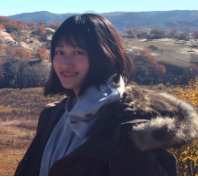
\includegraphics[width=1in,height=1in,clip,keepaspectratio]{./pic/jiawen}}]{Jiawen Zhang}
现为香港科技大学（广州）数据科学与分析方向博士生，导师为 Jia Li 教授。硕士毕业于中国科学院计算机技术专业，曾在微软亚洲研究院机器学习组担任研究实习生。研究兴趣包括数据挖掘与时间序列建模。
\end{IEEEbiography}
\vspace{-13 mm}

\begin{IEEEbiography}[{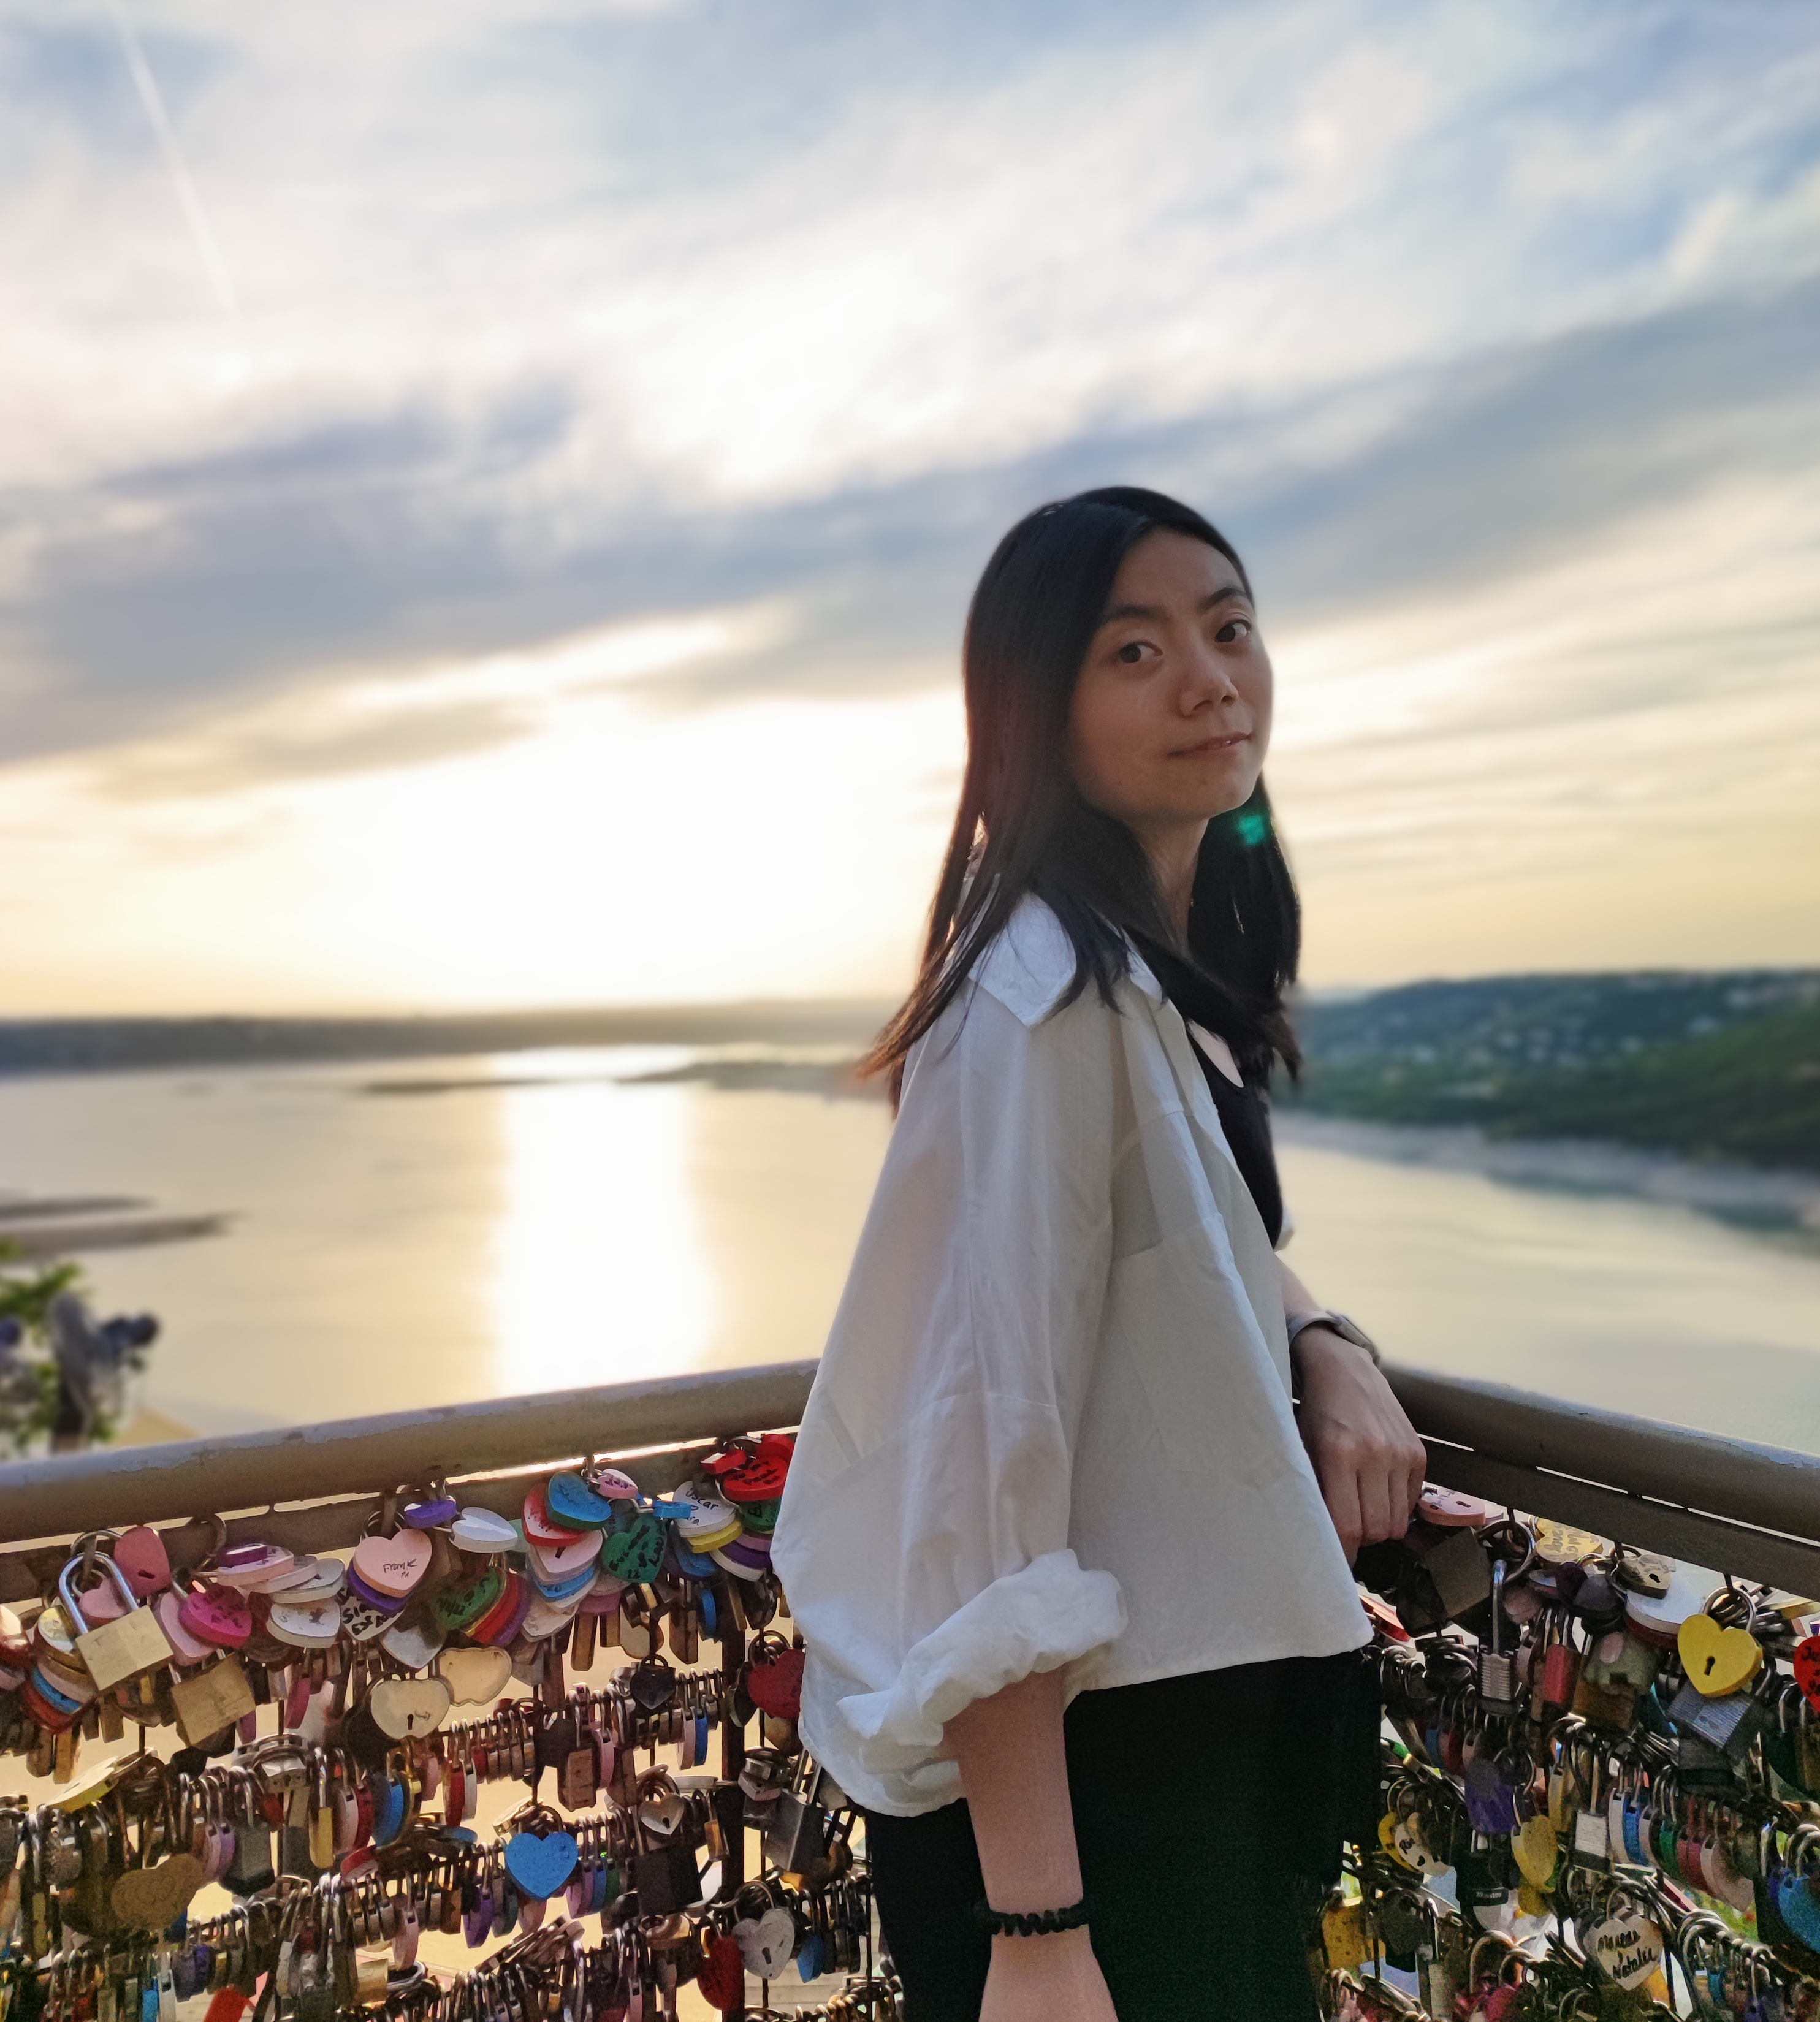
\includegraphics[width=1in,height=1in,clip,keepaspectratio]{./pic/xixi}}]{Xixi Wu}
现为复旦大学计算机科学学院硕士研究生（毕业年级）。2021 年获得复旦大学计算机科学学士学位。研究兴趣包括深度图学习、数据挖掘与推荐系统。已在 KDD/WWW/CIKM 等会议发表多篇第一作者论文。
\end{IEEEbiography}
\vspace{-13 mm}

\begin{IEEEbiography}[{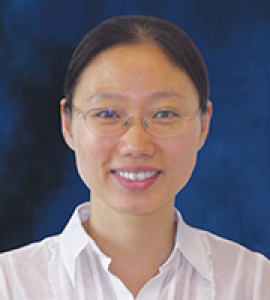
\includegraphics[width=1in,height=1in,clip,keepaspectratio]{./pic/hongcheng}}]{Hong Cheng}
现为香港中文大学系统工程与工程管理学系教授。2008 年获美国伊利诺伊大学厄巴纳—香槟分校博士学位。研究兴趣包括数据挖掘、数据库系统与机器学习。曾获 ICDE'07、SIGKDD'06 与 SIGKDD'05 等会议论文奖，并获得 2009 SIGKDD Doctoral Dissertation 证书表彰。曾获香港中文大学 2010 Vice-Chancellor's Exemplary Teaching Award。
\end{IEEEbiography}
\vspace{-10 mm}

\begin{IEEEbiography}[{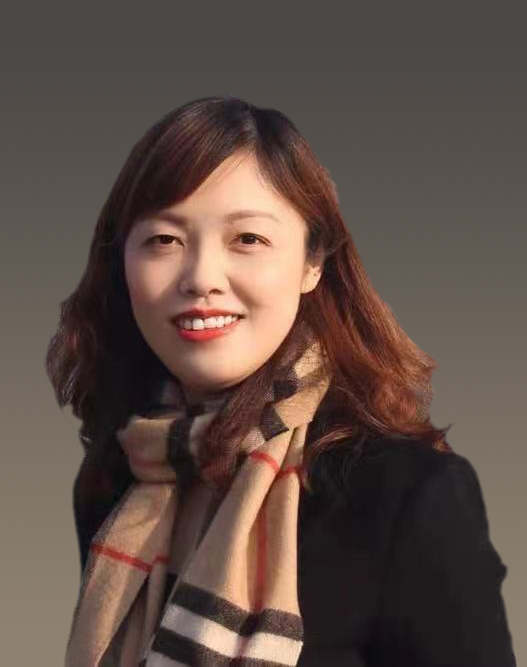
\includegraphics[width=1in,height=1in, clip,keepaspectratio]{./pic/yunxiong.jpg}}]{Yun Xiong}
现为复旦大学计算机科学学院、上海市数据科学重点实验室教授。2008 年获复旦大学博士学位。研究兴趣包括大数据挖掘与数据科学。在数据挖掘领域国际顶级期刊与会议（包括 TKDE、KDD、WWW、AAAI 等）发表论文 50 余篇。
\end{IEEEbiography}
\vspace{-13 mm}

\begin{IEEEbiography}[{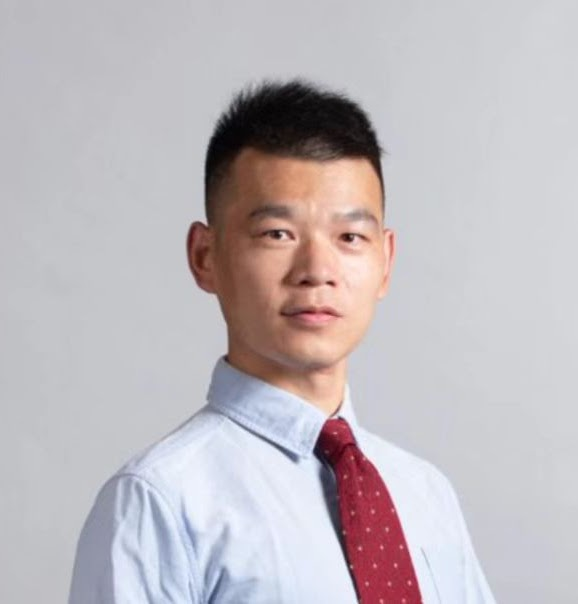
\includegraphics[width=1in,height=1in,clip,keepaspectratio]{./pic/jiali}}]{Jia Li}
现为香港科技大学（广州）助理教授。2021 年于香港中文大学获得博士学位。此前于 2014 至 2017 年在腾讯担任数据挖掘工程师，并于 2020 年在 Google AI（Mountain View）担任研究实习生。研究兴趣包括图学习与数据挖掘，相关工作发表于 TPAMI、ICML、NeurIPS、WWW、KDD 等重要期刊与会议。
\end{IEEEbiography}

\vfill
